\chapter{Evaluation of pilot jobs for Apache Spark applications on HPC
clusters}~\label{chp:spa} Val\'erie Hayot-Sasson and Tristan Glatard \\
\begingroup \footnotesize Department of Computer Science and Software
Engineering, Concordia University, Montreal, Canada \\
\endgroup 
\vspace{5pt} \\
Published in: \\
\hspace*{10pt} \textit{2019 15th International Conference on eScience
(eScience):} \url{10.1109/eScience.2019.00023}


\section{Abstract}
	Big Data has become prominent throughout many scientific fields, and as
	a result, scientific communities have sought out Big Data frameworks to
	accelerate the processing of their increasingly data-intensive
	pipelines. However, while scientific communities typically rely on
	High-Performance Computing (HPC) clusters for the parallelization of
	their pipelines, many popular Big Data frameworks such as Hadoop and
	Apache Spark were primarily designed to be executed on dedicated
	commodity infrastructures. This paper evaluates the benefits of pilot
	jobs over traditional batch submission for Apache Spark on HPC clusters.
	Surprisingly, our results show that the speed-up provided by pilot jobs
	over batch scheduling is moderate to non-existent (0.98 on average)
	despite the presence of long queuing times. In addition, pilot jobs
	provide an extra layer of scheduling that complicates debugging and
	deployment. We conclude that traditional batch scheduling should remain
	the default strategy to deploy Apache Spark applications on HPC
	clusters.
    
    
    \section{Introduction}
    
    Pilot jobs, also known as dynamic resource provisioning or glide-in
    scheduling, are a widely-used technique to address infrastructure
    heterogeneity, variable task queuing times, fine task granularity, and node
    failures on distributed computing infrastructures. Made popular by software
    projects such as Condor~\cite{thain2005distributed} and
    DIRAC~\cite{casajus2010dirac}, they became critical to grid computing,
    greatly improved the performance of HPC clusters, and enabled multi-cloud
    executions. 
    
    In contrast to static resource provisioning, pilot jobs are submitted to the
    infrastructure separately from the application, to provision resources on
    which application tasks will eventually be scheduled. Large pools of
    resources can thus be created, shielding applications from the underlying
    queuing times, failures, and other idiosyncrasies. A variety of frameworks
    now rely on pilot jobs, including RADICAL-Pilot~\cite{merzky2015radical},
    and recent versions of the Pipeline System for Octave and Matlab
    (PSOM)~\cite{bellec2012pipeline}. The survey
    in~\cite{turilli2018comprehensive} reviews the current pilot-job systems.
    
    % Goal of the paper
    In this paper, we study the use of pilot jobs to run scientific applications
    with Apache Spark~\cite{zaharia2016apache} on shared HPC clusters. The
    currently recommended method for this purpose involves batch requesting all
    the necessary resources and launching a Standalone Spark cluster once the
    resources have been allocated. This is, for instance, the method used on
    Compute Canada, our national computing infrastructure. With pilot jobs,
    rather than requesting all the resources at once, a Spark cluster is
    launched with a subset of the resources, and is expanded as more resources
    get allocated. Consistently with previous examples of pilot job deployments,
    we hypothesize that this strategy would reduce queuing times by (1)
    fragmenting resource requirements, and (2) allowing shorter wall-time
    estimates. While there have been some efforts on implementing pilot jobs for
    Apache Spark~\cite{luckow2016hadoop}, research is limited and none of them
    detail their quantitative effect.
    
    Apache Spark is a popular Big Data framework, commonly used in both
    industrial and academic settings. Although it is a Scala-based framework, it
    also has APIs for Java, Python (PySpark) and R. Spark's Resilient
    Distributed Dataset (RDD) abstraction enabled in-memory processing of
    pipelines by co-locating tasks and data, which provided important
    performance improvements compared to its predecessor Hadoop
    MapReduce~\cite{dean2008mapreduce}. Through the use of RDDs, it also became
    possible to execute iterative workflows -- something not easily doable in
    older frameworks. Schedulers for Spark include its built-in Standalone
    scheduler, Yet Another Resource Negotiator (YARN~\cite{apache13yet}), and
    Mesos~\cite{hindman2011mesos}. As a result of the sustained growth in data
    volumes, Apache Spark and other Big Data engines are increasingly used for
    scientific applications, including in neuroimaging, our primary field of
    interest~\cite{boubela2016big,mehta2017comparative,freeman2014mapping}.
    
    
    Big Data frameworks were designed with dedicated commodity infrastructure in
    mind, and, with the exception of Dask~\cite{rocklin2015dask}, do not support
    batch HPC schedulers such as the
    \href{http://www.univa.com/products/}{Oracle Grid Engine (OGE)},
    \href{https://slurm.schedmd.com/}{Slurm} and
    \href{https://www.adaptivecomputing.com/products/torque/}{TORQUE}, which are
    commonly available to scientists. Therefore, to run Big Data applications on
    HPC schedulers, it is also necessary to start an overlay cluster that will
    schedule application tasks on resources provisioned through batch
    schedulers. Our experiments quantify the effect of pilot jobs when combined
    with such an overlay cluster.
    
    To summarize, our paper makes the following contributions:
    \begin{itemize}
    \item We present SPA, a lightweight pilot-job framework to run Apache Spark
    applications on HPC clusters.
    \item We compare the makespan of a typical neuroimaging Big Data application
    with and without pilot jobs on two different HPC clusters and in different
    conditions.
    \item We describe a simple performance model to validate that the observed
    differences come from variations in queuing times rather than other factors.
    \end{itemize}
    Our methods, including infrastructure, job templates, application and
    performance model are described in Section~\ref{spa:sec:methods}.
    Section~\ref{spa:sec:results} presents our results which are discussed in
    Section~\ref{spa:sec:discussion}. Section~\ref{spa:sec:conclusion} concludes on
    the relevance of pilot jobs for Apache Spark applications on HPC clusters.
    
    \section{Materials and Methods}\label{spa:sec:methods}
    
	The application, templates, configuration files, benchmarks and analysis
	scripts are publicly available and can be found in our Spark Pilot-job
	scheduler for HPC Applications (SPA) repository at:
	\href{https://github.com/big-data-lab-team/spa}{https://github.com/big-data-lab-team/spa}.
	Links to the processing engines and processed data are provided in the
	text.
	
	\subsection{Infrastructure}
	All experiments were conducted on the Cedar and B\'eluga HPC computing
	clusters made available by \href{https://www.computecanada.ca}{Compute
	Canada} through \href{https://www.westgrid.ca}{WestGrid} and
	\href{http://www.calculquebec.ca}{Calcul Qu\'ebec}. Both clusters are
	accessible through the Slurm batch scheduler and Lustre parallel file
	system~\cite{schwan2003lustre}. The Cedar cluster has a total of 1542
	nodes with a total of 58,416 CPU cores. Available memory on a Cedar node
	can range from 125 to 3022~GB. Standard nodes are equipped with either 2
	Intel E5-2683 v4 Broadwell @ 2.1~Ghz (32 cores total) or 2 Intel
	Platinum 8160F Skylake @ 2.1Ghz (48 cores total) CPUs and 2 480~GB SSD.
	All nodes and temporary storage on Cedar are connected by an Intel
	OmniPath (version 1) with 100Gbit/s bandwidth.
    
	B\'eluga, on the other hand, is a smaller cluster with 872 available
	nodes. Node memory can range between 92 to \SI{752}{\giga\byte}, with
	the most common node type having \SI{186}{\giga\byte}. All nodes contain
	2 Intel Gold 6148 Skylake @ 2.4~Ghz (40 cores/node) CPU and are
	connected to each other with a 100~Gb/s Mellanox Infiniband EDR network.
	Each non-GPU node type contains one 480~GB SSD. 
    
	It is important to note that these clusters were used in production.
	That is, concurrently with other users. This allowed us to test the
	added-value of pilot scheduling in different realistic conditions of
	queuing times. At the time of our experiments, B\'eluga had recently
	been commissioned, resulting in low usage and shorter queuing times
	overall. Conversely, Cedar had been operating for a few years, resulting
	in higher usage and longer queuing times. We repeated our experiments
	multiple times in each configuration to capture queuing time
	variability.
    
	\subsection{Spark Configuration}
    
	There are three possible cluster managers available to use with Spark
	applications: the Standalone cluster manager, YARN and Mesos. The
	Standalone cluster manager is the most basic cluster manager available
	and is packaged directly with Spark. The YARN resource manager is
	designed for the resource management of Hadoop applications, however, it
	can be used with different types of applications as well. In contrast,
	Mesos was designed to manage the resources for a variety of
	applications. As such, it incorporates strategies that are more
	efficient for use with different frameworks making it possible to be
	used as an HPC scheduler. Due to Standalone's lightweight nature and our
	intent to start Spark clusters per application, we utilized the
	Standalone cluster manager.
    
	A Spark cluster is made up of three components: the cluster manager,
	workers and driver. The cluster manager, also known as the Spark master
	in Standalone mode, is responsible for the resource provisioning within
	the cluster.  As it is the resource manager for a given cluster, the
	cluster manager is not application specific. The driver requests
	resources from the master to launch its tasks. The master then
	dispatches the requests to workers with the necessary resources
	available to start executors. The driver may subsequently communicate
	with the executors to schedule and launch its tasks. Both the driver and
	the executors are application specific and connected directly to the
	master. 
    
	Spark has many configuration options available for dynamic resource
	provisioning. Its standalone cluster provides two deployment modes:
	client and cluster. The client deploy mode executes the driver within
	the \texttt{spark-submit} process as a client to the cluster. The
	cluster deploy-mode, however, runs the driver within a worker process.
	Such a configuration is practical when the driver program is deployed on
	a machine not co-located in the cluster to reduce network latency
	between workers and the driver. The cluster deploy mode also has the
	\texttt{supervise} feature which allows the driver to be restarted in
	case of failure. This is particularly useful for pilot-based overlay
	clusters where the running driver may fail due to wall-time expiration.
	Using the Standalone cluster manager, client mode is supported in all
	APIs, whereas cluster mode is only available for applications using the
	Scala, Java and R APIs.
    
	With HPC clusters, client mode is not necessarily possible on the login
	node as the driver client may require more resources than permitted.
	Moreover, due to cluster security policies, it may be difficult or
	impossible to execute the driver from an external computer, such as a
	personal laptop. Therefore, for both batch and pilot scheduling, it is
	necessary to launch the driver from within the Slurm jobs. That is, in
	cluster mode.
    
	Spark also provides master fault tolerance through single-node recovery
	wherever a shared file system is available. To enable this, a recovery
	folder must be set. Should the master fail, a new master will be able to
	take over based on the information available in the recovery folder.
    
	In long-running applications, it is necessary to be able to recover
	application execution from last successful state. Spark provides a
	checkpointing mechanism in order to ensure that the application is
	fault-tolerant to any kind of non application-related failure, such as a
	system failure.
    
	\subsection{SPA system design}
    
	There is no shortage of scripts available online for starting a Spark
	cluster on HPC, see for instance
	\href{https://github.com/NIH-HPC/spark-slurm}{spark-slurm},
	\href{https://www.sherlock.stanford.edu/docs/software/using/spark}{scripts}
	provided by Stanford's Sherlock cluster,
	\href{https://sparkhpc.readthedocs.io}{sparkhpc}, or
	\href{https://www.osc.edu/~troy/pbstools/man/pbs-spark-submit}{pbs-spark-submit}.
	However, all these scripts start up a cluster within a single batch
	call. At most, there are two calls, one for cluster startup, and the
	other, to launch the application. None of these use any kind of
	pilot-scheduling approach, nor do they discuss the effects of queuing
	time and how they might want to adjust it in the case where the driver
	is started separately from the batch job to start the cluster. Even in
	the case of RADICAL-Pilot, as per some available tutorials for using the
	pilot-job application with Spark (see
	\href{https://github.com/radical-cybertools/pilot-streaming/blob/master/examples/Pilot-Streaming-GettingStarted.ipynb}{here}
	and
	\href{https://github.com/radical-cybertools/MIDAS-tutorial/blob/master/pilot/Pilot-Spark.ipynb}{here}),
	it appears that the Spark cluster is started within a single pilot and
	the application is submitted, in a separate process, to that pilot. Due
	to the fact that existing solutions mainly rely on a single batch call
	to start up the Spark cluster and do not appear to be able to submit
	multiple smaller jobs to improve queuing times, we have decided to
	implement our own solution for the sake of our experiments.
    
	Two different job templates were developed to implement the two main
	conditions compared in our experiments: the batch submission template
	and the pilot submission template. The batch submission template was
	inspired by the template provided by Compute Canada to launch Spark
	applications on Slurm,
	\href{https://docs.computecanada.ca/wiki/Apache\_Spark/en}{available
	here}. The template operates as follows: certain resource requirements
	are requested by the user (e.g. wall-time, amount of memory per node,
	number of CPUs per task, number of nodes and number of tasks per node).
	Once these resources are allocated, a master is started on one of the
	requested node resources. Then, after the master has successfully
	started, the workers are started on all nodes. Multiple worker instances
	are started on a single node by setting the
	\texttt{SPARK\_WORKER\_INSTANCES} environment variable to the number of
	tasks per node. Each worker is given as many cores as specified by the
	user in the Slurm resource allocation request. After both the masters
	and the workers have successfully started, the driver is finally
	started. The amount of memory given to each executor corresponds to 95\%
	of the available memory on the node, to allow for offheap space. The
	Spark deploy mode selected for the batch template is client mode. We
	selected this deploy mode over cluster mode as driver recovery would not
	be required in batch in the case of wall-time expiration, as all the
	allocated resources will expire at the same time. Moreover, many
	scientific applications are written in Python, which cannot use cluster
	mode using the Standalone resource manager. Should pilot scheduling
	using cluster mode significantly reduce queuing time compared to batch
	scheduling using client mode, it would provide enough justification to
	extend Spark's Standalone scheduler to include cluster mode for PySpark
	applications.
    
	The pilot submission template is similar to that of the batch template,
	although, each pilot will start its own Spark master and worker.
	However, there will only be one pilot which will start the driver
	process. The pilot selected to start the driver is the first one that
	attempts to do so by means of a lockfile. The reason for which each
	pilot starts its own master is to ensure the fault tolerance of the
	masters. In this configuration, should the active master be killed, one
	of the stand-by masters can take over and the application may be able to
	resume if single-node recovery is set. Such a configuration is
	particularly favourable in pilot scheduling scenarios as node failures
	may be more frequent due to wall-time expiration. Additionally, the
	Spark deploy mode of the driver was selected to be cluster deploy mode.
	This would not only allow the driver to be executed directly on one of
	the workers, but also allow us to make the driver fault-tolerant through
	the \texttt{supervise} mode, which is only available in cluster deploy.
	As with the masters, it is particularly important to have a
	fault-tolerant driver in pilot-scheduling scenarios due to possible
	wall-time expiration. Should pilots be idle for a certain duration, the
	pilots will terminate themselves in order to not hog resources.
	% \TG{It should be explained before that one of the interests of pilots
	% is to ``play'' with shorter wall-times}. \TG{It would also be nice to
	% have runs where pilots have shorter wall-times, to see if queuing
	% times are shorter too.}
    
	Although we start a master on each pilot, we have not incorporated the
	master recovery function for our experiments. However, this feature is
	important and should be incorporated in pilot schedulers where any nodes
	can fail by design.
    
	Due to the differences in deploy modes between batch and pilot
	submission, batch will always inevitably have one more worker than
	pilot. This is because in cluster deploy, which pilot uses, the driver
	occupies a worker, whereas in client deploy, the driver is a distinct
	process.
    
	Both of these Slurm templates are launched within a Python application
	called \textit{SPA}. The templates are used in conjunction with JSON
	configuration file and passed to the
	\href{https://github.com/brentp/slurmpy}{SlurmPy} library within
	\textit{SPA}. The \textit{SPA} application ensures that all is
	preconfigured correctly before passing it to SlurmPy. It also ensures
	that enough pilots are launched, maintains track of the running/queued
	pilots, and launches additional pilots if there are fewer pilots than
	requested by the user in the Slurm queue.
    
	\subsection{Application}
	    \begin{algorithm}\caption{Incrementation}\label{spa:alg:incrementation}
	    
		\SetKwInOut{Input}{Input} \Input{$x$ a sleep delay in seconds;\\
			$n$ a number of iterations;\\
			$c$ a set of image chunks;\\} \ForEach{$chunk$ in $c$}{
		    
			read $chunk$\;                                        
			\For{$i \in \llbracket 1, n \rrbracket$}{
			
			    $chunk\gets chunk+1$\;
			    
			    sleep $x$\;                          
			}
			
			write $chunk$\;
			
		    }
		    
	    \end{algorithm}
	To determine the added value of pilot over batch scheduling of Spark
	applications, we required a Spark application operating on a large
	dataset with an important processing time to emulate what would be the
	average requirements of a scientific Spark application. For this, we
	created a synthetic application that would process the 40~$\mu$m
	BigBrain~\cite{amunts2013bigbrain}, a \SI{76}{\giga\byte} 3D
	histological image of a human brain. The algorithm is a chain of map
	transformations that, at each transformation, increment the voxels of
	the image by 1 (see Algorithm~\ref{spa:alg:incrementation}). We selected
	a synthetic algorithm as the focus of our experiments is pilot
	scheduling and not the application in and of itself. Furthermore, this
	algorithm enabled us to have control over the task duration and make it
	representative of scientific applications. Additionally, it was
	important that the overall application duration did not vary between the
	different levels of parallelism within our experiments. Being able to
	adjust the task duration based on level of parallelism allowed us to
	achieve this.
    
	Spark cluster fault-tolerance is important in determining the
	suitability of pilot-jobs for Spark applications on HPC. Executing jobs
	on a shared cluster may result in a variety of failures. Pilot jobs may
	be more likely to fail as a result of underestimation of resources (e.g.
	wall-times), and therefore, should be fault-tolerant to master, worker
	and driver failures. Although built-in fault-tolerance was not
	investigated in this paper, we want to ensure that the environment is
	set up in such a way that Spark's fault-tolerance configuration could
	easily be set should our experiments return favourable results for
	pilot-jobs. Fault-tolerance of the driver is only possible in cluster
	deploy mode, however, when using Spark's Standalone scheduler, this mode
	is not available for Python applications. It is for this reason that our
	synthetic application is written in Scala. Nevertheless, cluster deploy
	mode is available for PySpark applications using YARN or Mesos
	schedulers.
    
    
	\subsection{Performance model}
    
	The makespan of an application is defined as the total duration between
	the submission time of the first application task, and the completion
	time of the last application task. It includes any scheduling time,
	queuing time, data transfer time, and any other overhead.
	
	Assuming a divisible load, i.e., the application can be divided in any
	number of tasks, the makespan can be written using the following
	expression, which holds for both batch and pilot execution modes:
	\begin{equation}
	    M = \frac{C}{W} \label{eq:mcw}
	\end{equation}
	where:
	\begin{itemize}
	    \item $M$ is the makespan of the application
	    \item $C$ is the total execution time of the application
	    \item $W$ is the \emph{average} number of Spark workers throughout
	    the execution
	\end{itemize}
	The average number of workers $W$ allows the model to take into account
	 variable queuing times. It is computed as follows:
	\begin{equation}
	    W = \frac{1}{M}\int_0^M{w(t)dt}\label{eq:spa:avgw}
	\end{equation}
	where $w(t)$ is the number of workers available at time $t$. When the
	application is not subject to any scheduling or queuing time, the
	average number of workers equals the number of workers requested. 
    
	Therefore, assuming a fixed total execution time, the relation between
	batch and pilot jobs can be represented as:
	\begin{equation}
	    \frac{M_{batch}}{M_{pilot}} = \frac{W_{pilot}}{W_{batch}}\label{eq:spa:makespancomp}
	\end{equation}
	where:
	\begin{itemize}
	    \item $M_{batch}$ is the makespan of the batch application
	    \item $M_{pilot}$ is the makespan of the pilot application
	    \item $W_{pilot}$ is the average number of workers of the pilot
	    application
	    \item $W_{batch}$ is the average number of workers of the batch
	    application
	\end{itemize}
	We will use this relation to discuss our results later on. It
	corresponds to an ideal case where no data or other overhead is present:
	only queuing times are included, through the integration in
	Equation~\ref{eq:spa:avgw}.
    
	\subsection{Added value of pilot scheduling}
	    \begin{table}                                                                    
		\centering                                                                       
		\begin{tabular}{c|c|c|c}                                                             
		\rowcolor{headcolor}                                                             
		Configuration & RAM (GB) & Tasks & Cores per task\\
		
		\hline                                                                           
		1 & 112 & 16 & 1\\
		
		2 & 224 & 32 & 1\\
		
		3 & 336 & 48 & 1\\
		4 & 448 & 64 & 1\\
		\end{tabular}                                                                    
		\setlength{\belowcaptionskip}{-10pt}                                             
		\caption{Resource configurations}                                                    
		\label{table:spa:dedicatednodes}                                                            
	    \end{table} 
	       
	    \begin{table*}                                                                   
	    \centering                                                                       
	    
	   \resizebox{\columnwidth}{!}{%
	    \begin{tabular}{c|cccccc}                                                   
	      \rowcolor{headcolor}                                                           
	      \multicolumn{7}{c}{Configuration 1}\\                      
	      \hline                                                                         
	      \rowcolor{headcolor}                                                           
	      Execution mode & Nodes/job & RAM (GB) & CPUs per task & Tasks/node
	      & Walltime & Task delay (s) \\                             
	      \hline
	      Batch & 1 & 112 & 1 & 16 & 2h30 & 45 \\
	      8 pilots & 1 & 14 & 1 & 2 & 2h30 & 45 \\
	      16 pilots & 1 & 7 & 1 & 1 & 2h30 & 45 \\
    
	      \hline                                                                           
	      \multicolumn{7}{c}{}\\
	      
    
	      \rowcolor{headcolor}                                                           
	      \multicolumn{7}{c}{Configuration 2}\\                      
	      \hline                                                                         
	      \rowcolor{headcolor}                                                           
	      Execution mode & Nodes/job & RAM (GB) & CPUs per task & Tasks/node
	      & Walltime & Task delay (s) \\                             
	      \hline
	      Batch & 2 & 112 & 1 & 16 & 2h30 & 90 \\
	      8 pilots & 1 & 28 & 1 & 4 & 2h30 & 90 \\
	      16 pilots & 1 & 14 & 1 & 2 & 2h30 & 90 \\
    
	      \hline                                                                           
	      \multicolumn{7}{c}{}\\
	      
    
	      \rowcolor{headcolor}                                                           
	      \multicolumn{7}{c}{Configuration 3}\\                      
	      \hline                                                                         
	      \rowcolor{headcolor}                                                           
	      Execution mode & Nodes/job & RAM (GB) & CPUs per task & Tasks/node
	      & Walltime & Task delay (s) \\                             
	      \hline
	      Batch & 3 & 112 & 1 & 16 & 2h30 & 120 \\
	      8 pilots & 1 & 42 & 1 & 6 & 2h30 & 120 \\
	      16 pilots & 1 & 21 & 1 & 3 & 2h30 & 120 \\
    
	      \hline                                                                           
	      \multicolumn{7}{c}{}\\
	      
    
	      \rowcolor{headcolor}                                                           
	      \multicolumn{7}{c}{Configuration 4}\\                      
	      \hline                                                                         
	      \rowcolor{headcolor}                                                           
	      Execution mode & Nodes/job & RAM (GB) & CPUs per task & Tasks/node
	      & Walltime & Task delay (s) \\                             
	      \hline
	      Batch & 4 & 112 & 1 & 16 & 2h30 & 180 \\
	      8 pilots & 1 & 56 & 1 & 8 & 2h30 & 180 \\
	      16 pilots & 1 & 28 & 1 & 4 & 2h30 & 180 \\
    
	      \hline                                                                           
	      \multicolumn{7}{c}{}\\
	      
	    \end{tabular}
	    }                                                                  
	    \setlength{\belowcaptionskip}{-10pt}                                             
	    \caption{Experimental conditions}
	    \label{table:spa:conditions}                                                        
	    \end{table*}                                                                                   
	    To determine if there are any performance benefits to using pilot
	    over batch scheduling, we needed to compare both strategies given
	    various resource requirements. It is expected that large batch
	    requests will stay in the resource queue longer than multiple pilot
	    requests that ultimately use up the same amount of resources, as
	    each individual pilot requests fewer resources at a time. We
	    therefore used four resource configurations to investigate this
	    hypothesis (Table~\ref{table:spa:dedicatednodes}).
    
	   For batch, we requested 1 to 4 dedicated nodes, depending on resource
	   configuration, each with 112~GB of RAM, 1 core per task and 16 tasks
	   per node. On the other hand, for all configurations, we ran our
	   experiments with 8 and 16 pilots. Experimental conditions can be seen
	   in Table~\ref{table:spa:conditions}.
    
	   As the focus of our experiments is to measure the impact pilot
	   scheduling has on queuing times, we wanted to ensure that our
	   wall-time estimates would be consistent for each experimental
	   condition. Therefore, we adjusted task delay based on the maximum
	   level of parallelism to ensure that wall-times would not need to be
	   readjusted for each configuration. Given utmost parallelism, the
	   sleep delay added would amount to a makespan of 1 hour regardless of
	   configuration. The actual processing time of the application,
	   however, would differ between configurations as we did not account
	   for task duration (incrementation time, line 8 in
	   Algorithm~\ref{spa:alg:incrementation}) in the sleep delay. Due to
	   slight variability in task durations between experiments, in addition
	   to variability in application parallelism due to queuing times of
	   each pilot Slurm job, we set the Slurm allocation wall-time to be
	   2h30 to ensure experiment completion.
    
	   For each configuration, all three execution modes (batch, 8 pilots,
	   16 pilots) were executed in parallel to ensure that the status of the
	   HPC cluster was the same when the different execution modes were
	   launched. Furthermore, the submission order of the execution modes
	   for each configuration was randomized to ensure that Slurm job
	   request order could not have affected results. 
    
	   There were 10 repetitions in total for each configuration, and the
	   order in which the configurations were launched was also randomized.
	   This was to account for any system variability that can occur,
	   particularly in production HPC clusters. 
    
	   Different clusters may have different resource configurations, number
	   of users and scheduling policies. Therefore, we executed all 10
	   repetitions on both Cedar and B\'eluga to determine how much our
	   results differ between two distinct clusters.
    
	% maybe remove \subsection{Pipeline robustness} While nodes failures can
	%occur for various reasons, underestimation of wall-time may lead to
	%early node termination in pilot scheduling systems. Therefore, it is
	%crucial for the overlay cluster within the pilot system to be robust to
	%node failures. In this series of experiments, we investigate Spark's
	%fault-tolerance with respect to worker, master and driver termination.
    
	%   In our configuration, the driver is running in cluster deploy-mode,
	%    resulting in it being executed directly on a worker. This feature
	%    alone should not make it fault-tolerant to failures. However, using
	%    this feature coupled with the \texttt{--supervise} flag, will. 
    
	% maybe remove\subsection{Checkpointing} \todo{metric for determining
	%    how often to checkpoint based on cluster size} maybe remove
	%    \subsection{Job arrays} \todo{need to kill idle workers. may not
	%    want all workers to be running at once.} maybe remove
	%    \subsection{Example application} \todo{incrementation with varying
	%    task durations}
    
    \section{Results}\label{spa:sec:results}
    
    As can be seen in both Figures~\ref{fig:spa:makespansbeluga}
    and~\ref{fig:spa:makespanscedar}, pilots generally did not bring any
    performance improvement to the execution of Spark workloads on either
    system. In B\'eluga and Cedar, 16 pilots were generally slower than batch
    except for a few occurrences. When 16 pilots were faster, it was generally
    either very slight, or, as expected, when batch queuing times were very
    large. The maximum speedup achieved was approximately 5.6$\times$ for 8 and
    16 pilots on B\'eluga and 2.6$\times$ on Cedar. It is only in
    Configuration~3 (Figure~\ref{fig:spa:beluga4}) on B\'eluga that we spot any
    large speedups, however, it generally remains that pilots are slightly
    slower, even in this configuration. The same can be said about Cedar,
    however, it occurred with Configuration~4 instead of 3. On average, pilots
    were up to 0.11$\times$ slower on B\'eluga and 0.17$\times$ slower on Cedar
    (see Table~\ref{table:spa:speedup}), both of which occurred when using 16
    pilots. The only times when pilots were found to be, on average, faster, was
    in Configuration~3 on B\'eluga and Configuration~4 on Cedar where the
    speedup was found to reach a max of 1.46 for 8 pilots on B\'eluga. The
    missing bars in Figures~\ref{fig:spa:makespansbeluga}
    and~\ref{fig:spa:makespanscedar} correspond to failed executions.
    
	\begin{figure*}
	    \centering
	    \begin{subfigure}[b]{0.475\textwidth}
		\centering
		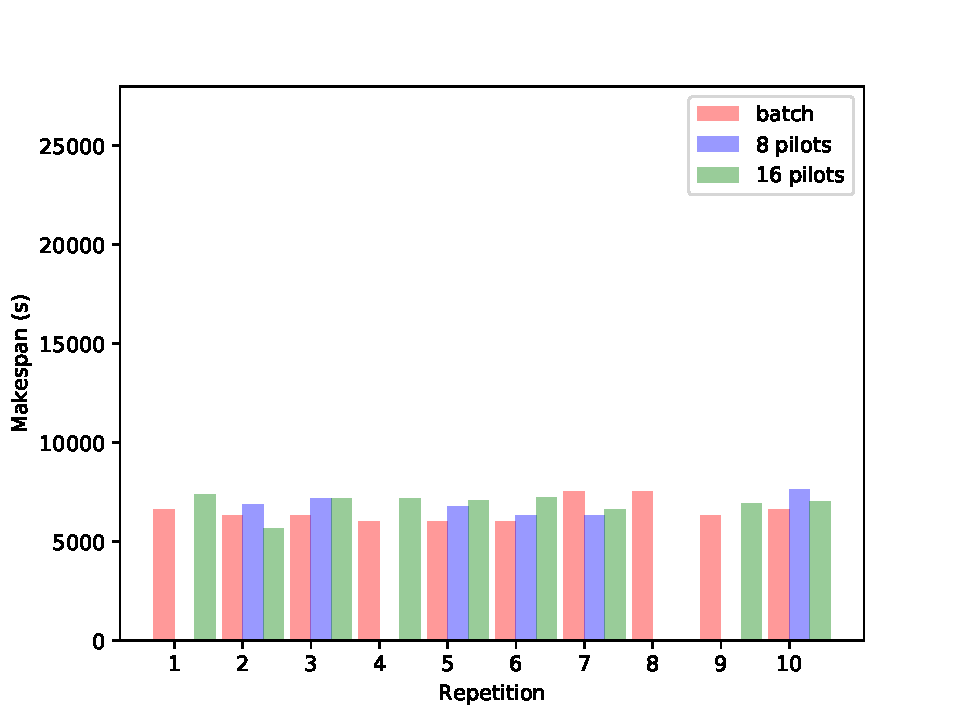
\includegraphics[width=\textwidth]{figures/spa/dedicated_1_beluga}
		\caption[]%
		{{\small Configuration 1}}
		\label{fig:spa:beluga1}
	    \end{subfigure}
	    \hfill
	    \begin{subfigure}[b]{0.475\textwidth}
		\centering
		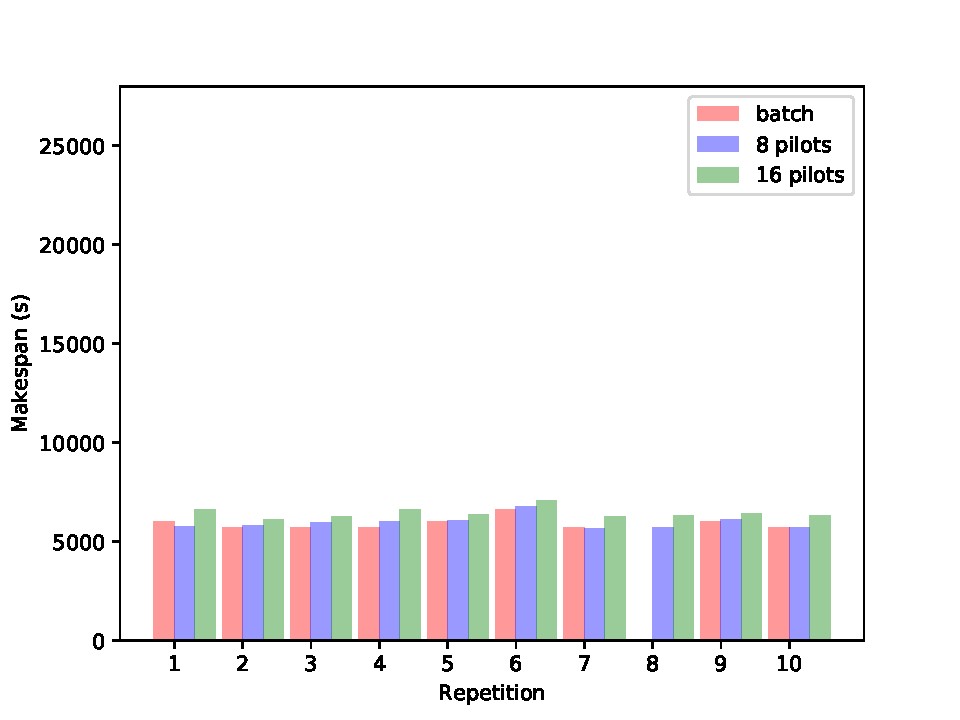
\includegraphics[width=\textwidth]{figures/spa/dedicated_2_beluga}
		\caption[]%
		{{\small Configuration 2}}
		\label{fig:spa:beluga2}
	    \end{subfigure}
	    \vskip\baselineskip
	    \begin{subfigure}[b]{0.475\textwidth}
		\centering
		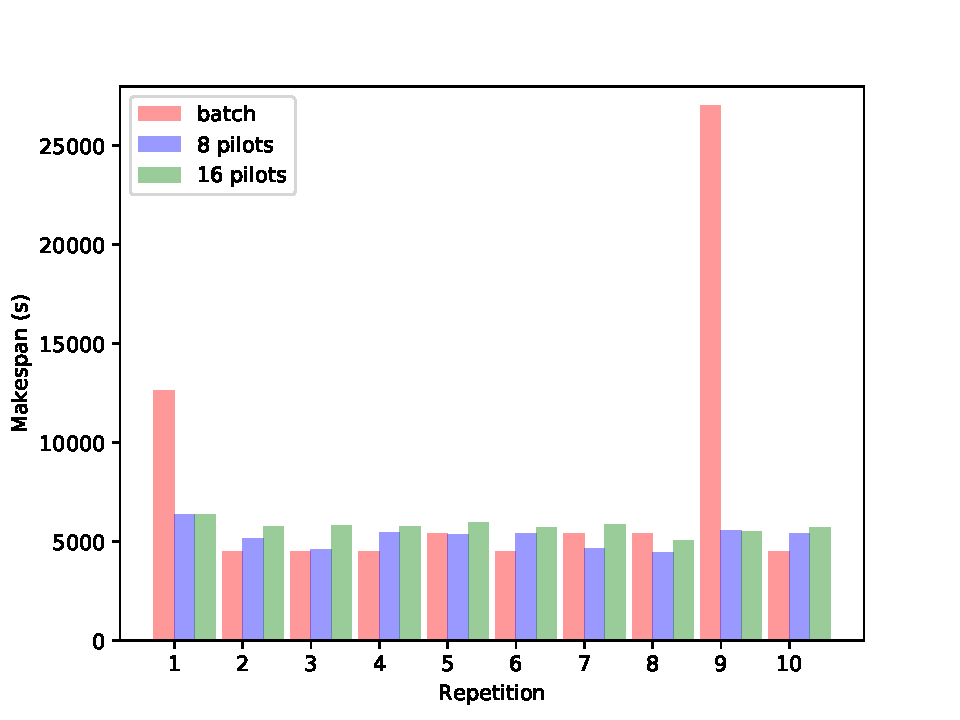
\includegraphics[width=\textwidth]{figures/spa/dedicated_3_beluga}
		\caption[]%
		{{\small Configuration 3}}
		\label{fig:spa:beluga3}
	    \end{subfigure}
	    \quad
	    \begin{subfigure}[b]{0.475\textwidth}
		\centering
		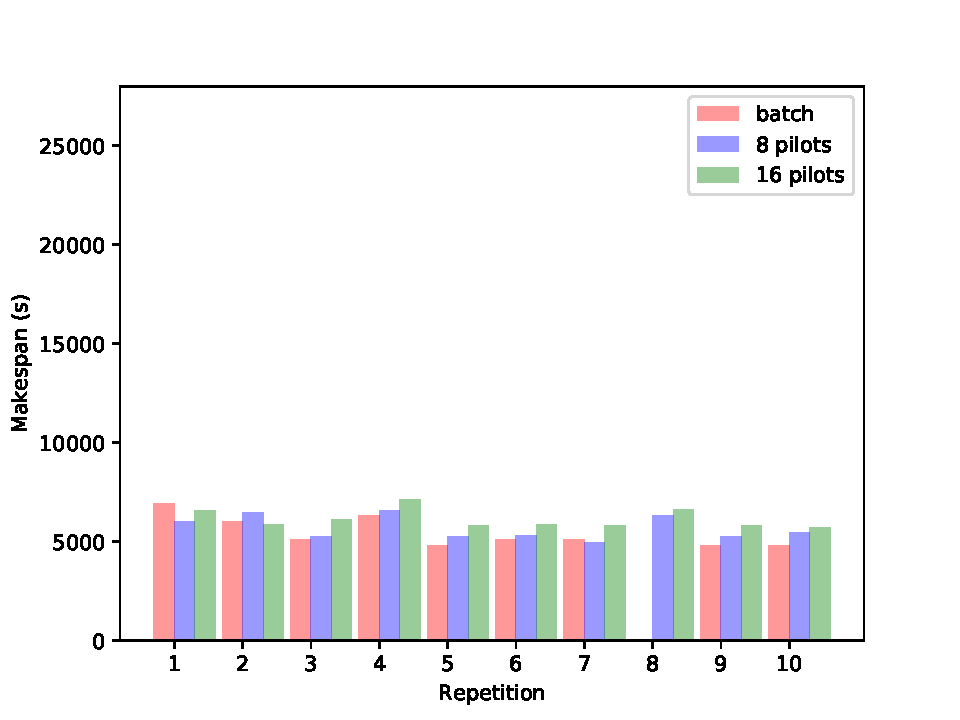
\includegraphics[width=\textwidth]{figures/spa/dedicated_4_beluga}
		\caption[]%
		{{\small Configuration 4}}
		\label{fig:spa:beluga4}
	    \end{subfigure}
	    \caption{\small The application makespan on the Beluga cluster for all repetitions.}
	    \label{fig:spa:makespansbeluga}
	\end{figure*}
    
    
	\begin{figure*}
	    \centering
	    \begin{subfigure}[b]{0.475\textwidth}
		\centering
		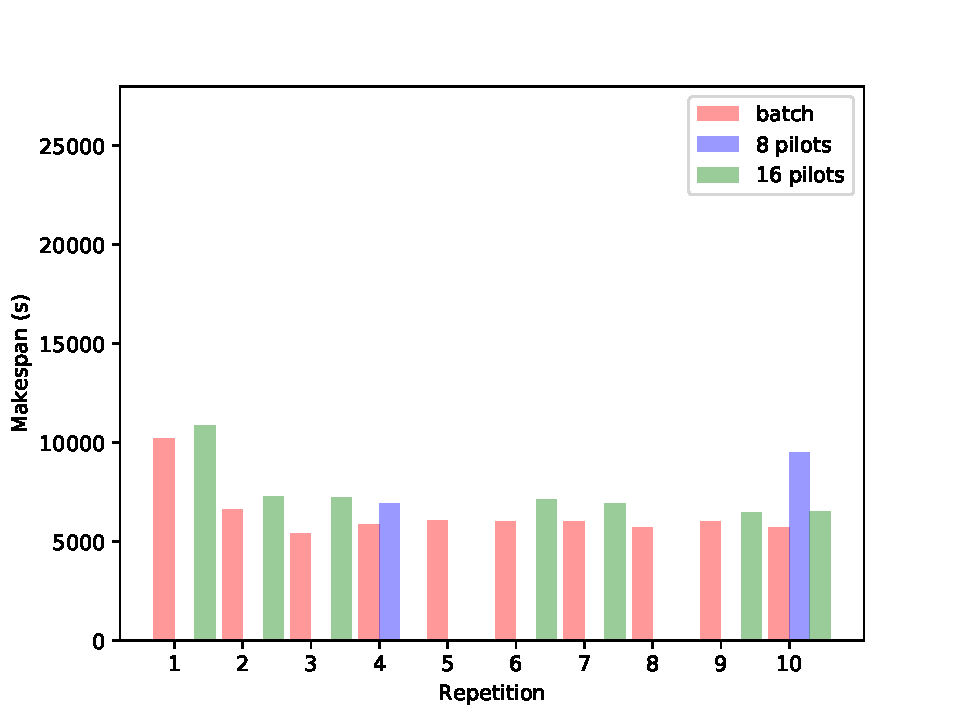
\includegraphics[width=\textwidth]{figures/spa/dedicated_1_cedar}
		\caption[]%
		{{\small Configuration 1}}
		\label{fig:cedar1}
	    \end{subfigure}
	    \hfill
	    \begin{subfigure}[b]{0.475\textwidth}
		\centering
		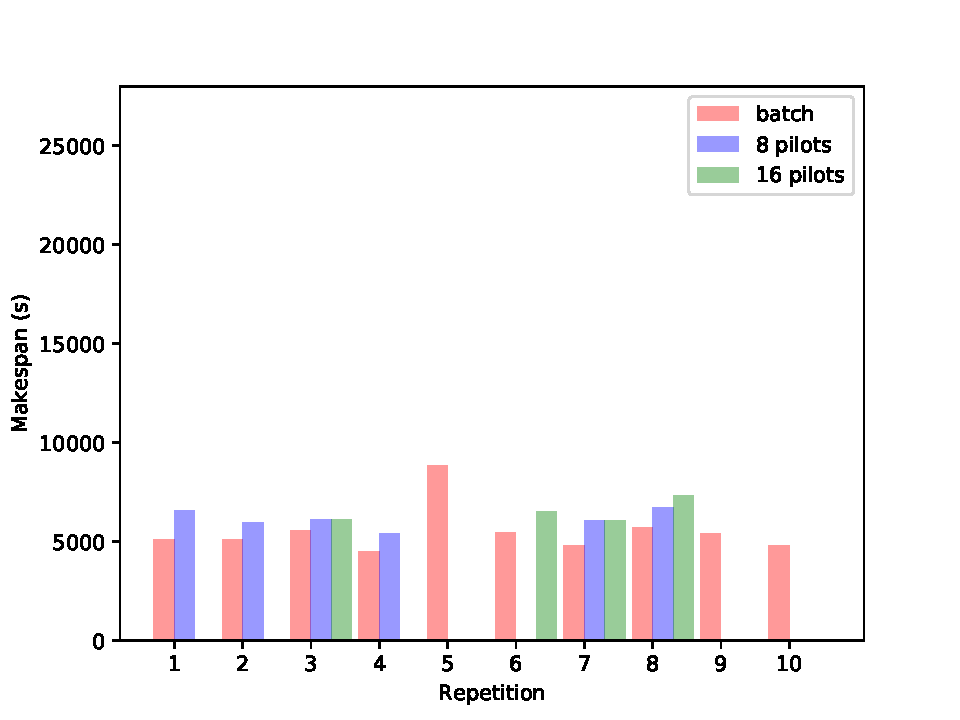
\includegraphics[width=\textwidth]{figures/spa/dedicated_2_cedar}
		\caption[]%
		{{\small Configuration 2}}
		\label{fig:cedar2}
	    \end{subfigure}
	    \vskip\baselineskip
	    \begin{subfigure}[b]{0.475\textwidth}
		\centering
		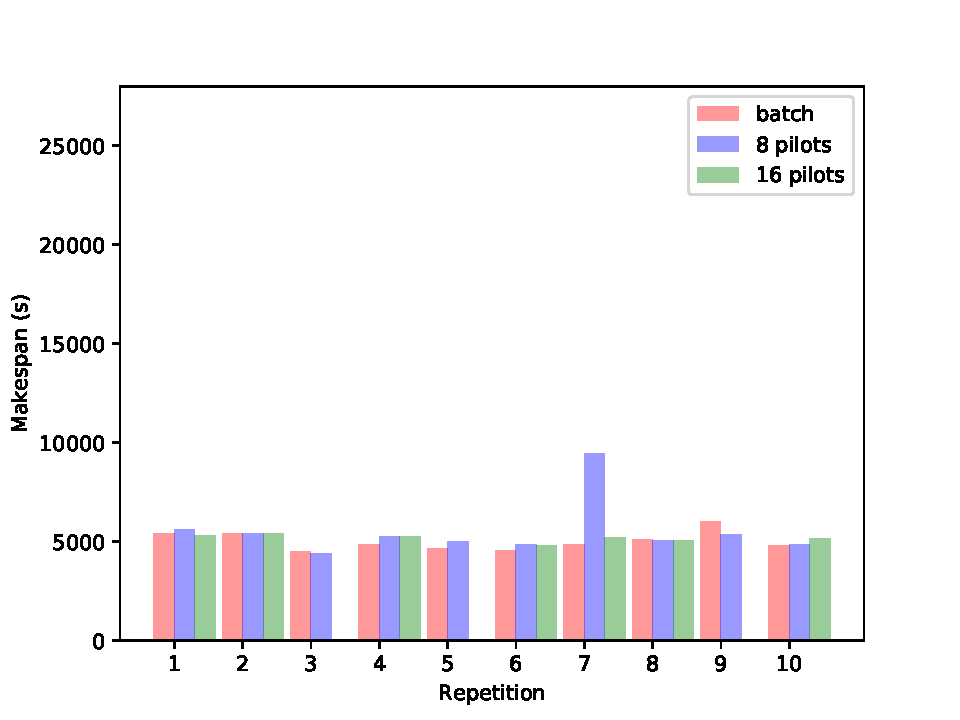
\includegraphics[width=\textwidth]{figures/spa/dedicated_3_cedar}
		\caption[]%
		{{\small Configuration 3}}
		\label{fig:cedar3}
	    \end{subfigure}
	    \quad
	    \begin{subfigure}[b]{0.475\textwidth}
		\centering
		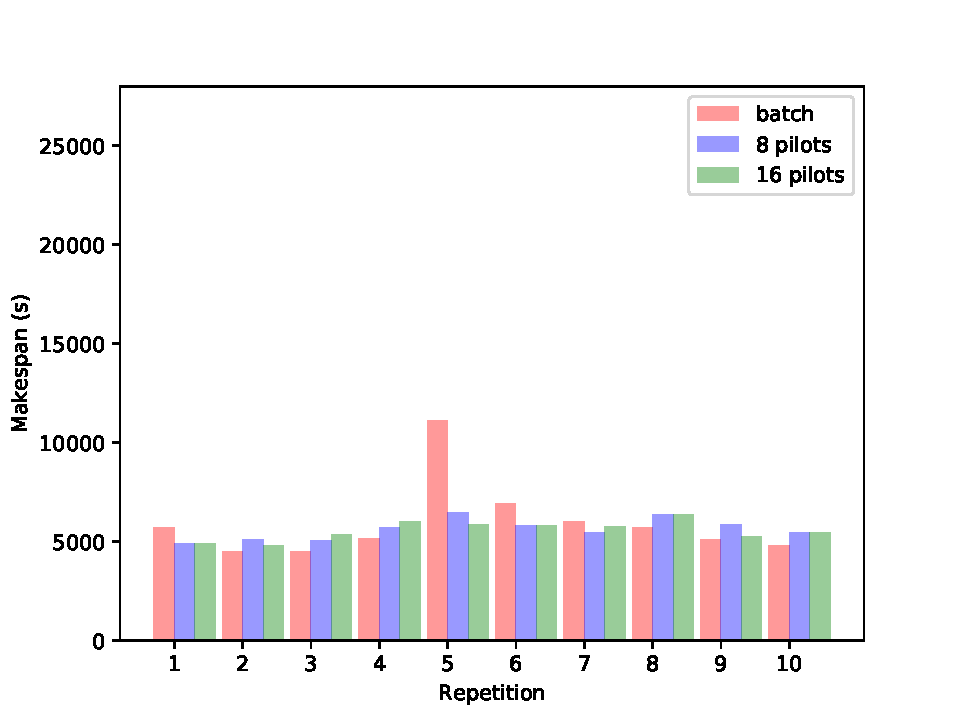
\includegraphics[width=\textwidth]{figures/spa/dedicated_4_cedar}
		\caption[]%
		{{\small Configuration 4}}
		\label{fig:cedar4}
	    \end{subfigure}
	    \caption{\small The application makespan on the Cedar cluster for all repetitions.}
	    \label{fig:spa:makespanscedar}
	\end{figure*}
    
    
    In the case of pilots, multiple Slurm jobs, each with potentially different
    queuing times, were used. Figure~\ref{fig:spa:mwall} displays the makespan
    times for an average number of workers given an experiment configuration,
    where the coloured line corresponds to the estimated makespan using our
    performance model. Makespan for the model was calculated as:
    $$
    M = \frac{125\times(d + 20)}{W}\times 10,
    $$
    where:
    \begin{itemize}
	\item $125$ is the number of chunks BigBrain was split into
	\item $M$ is the makespan of the application, in seconds
	\item $W$ is the average number of Spark workers throughout the
	execution, computed as in Equation~\ref{eq:spa:avgw}
	\item $d$ is the task delay, in seconds, associated with a given
	configuration
	\item $20$ is the average measured incrementation duration, in seconds,
	for a BigBrain chunk
	\item $10$ is the number of iterations
    \end{itemize}
    As can be seen in the Figure~\ref{fig:spa:mwall}, both pilots and batch
    followed the general trend denoted by the model, which confirms that the
    system was behaving without major external sources of overhead. However,
    pilots were consistently slower than batch for the same number of average
    workers. This is particularly visible in Configuration 4 on B\'eluga (Fig.
    \ref{fig:spa:mwbeluga}), and in Configuration 2, 3 and 4 on Cedar (Fig.
    \ref{fig:spa:mwcedar}). It means that some sort of overhead impacted pilots
    but not batch. It can also be noticed that both batch and pilots
    occasionally deviated from the model line, in particular Configurations 2
    and 3 in B\'eluga: this is due to the fact that our application is not a
    divisible load, as the model assumes. Extending the model beyond divisible
    loads is easy enough for batch and confirms that the observed deviations
    from the model line come from this assumption (see grey line in
    Fig.~\ref{fig:spa:mwall}). The extended expression for pilots is more
    complex though.
    
    When comparing the average number of worker difference
    (Figures~\ref{fig:spa:nworkersbeluga} and~\ref{fig:spa:nworkerscedar}), it
    can be seen that (1) repetitions where pilots were faster than batch
    correspond to repetitions where pilots had more workers, and vice versa --
    this confirms that performance differences are mainly coming from queuing
    time differences, and (2) pilot average number of workers start to exceed
    batch as the application requirements increase, that is, for Configuration 3
    and 4.
    
    \begin{figure*}
    
	    \centering
	    \begin{subfigure}[b]{0.475\textwidth}
		\centering
		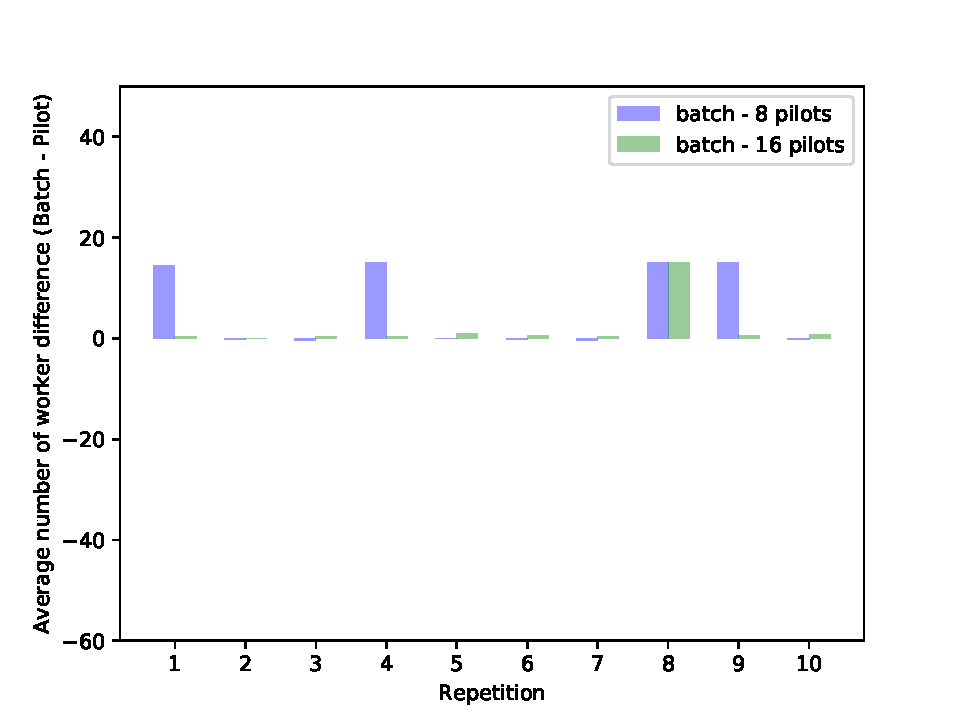
\includegraphics[width=\textwidth]{figures/spa/nworkers_1_beluga}
		\caption[]%
		{{\small Configuration 1}}
		\label{fig:spa:nwbeluga1}
	    \end{subfigure}
	    \hfill
	    \begin{subfigure}[b]{0.475\textwidth}
		\centering
		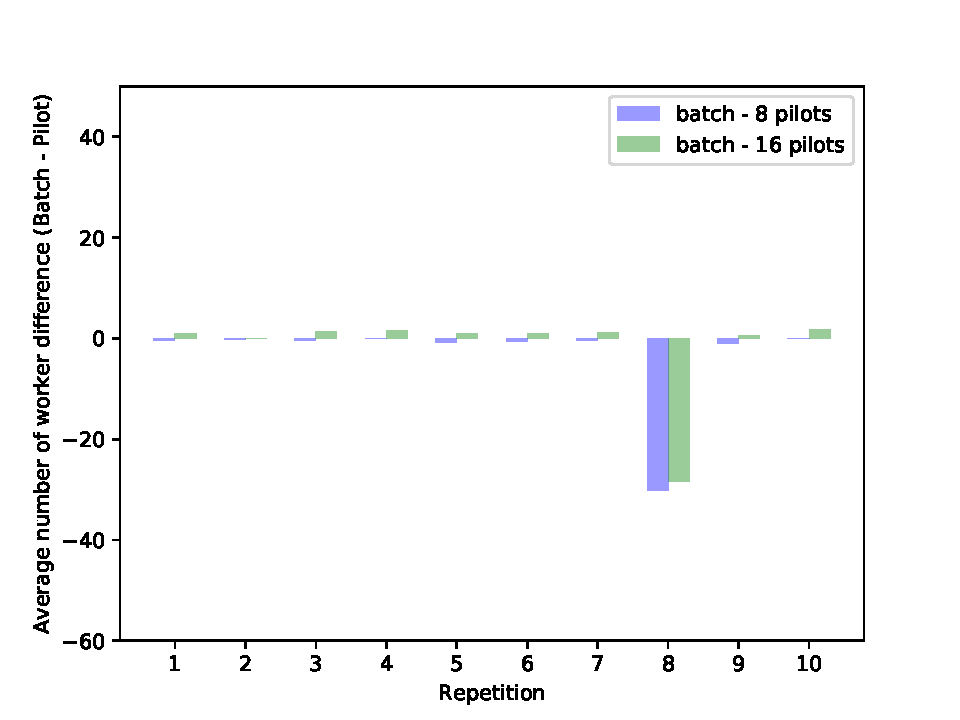
\includegraphics[width=\textwidth]{figures/spa/nworkers_2_beluga}
		\caption[]%
		{{\small Configuration 2}}
		\label{fig:spa:nwbeluga2}
	    \end{subfigure}
	    \vskip\baselineskip
	    \begin{subfigure}[b]{0.475\textwidth}
		\centering
		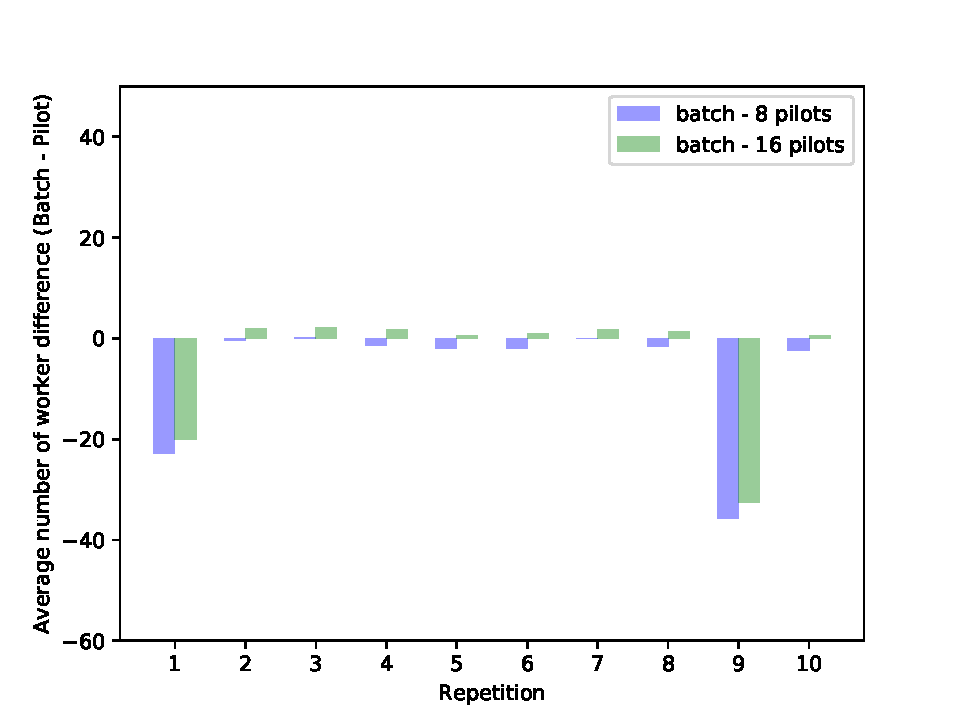
\includegraphics[width=\textwidth]{figures/spa/nworkers_3_beluga}
		\caption[]%
		{{\small Configuration 3}}
		\label{fig:spa:nwbeluga3}
	    \end{subfigure}
	    \quad
	    \begin{subfigure}[b]{0.475\textwidth}
		\centering
		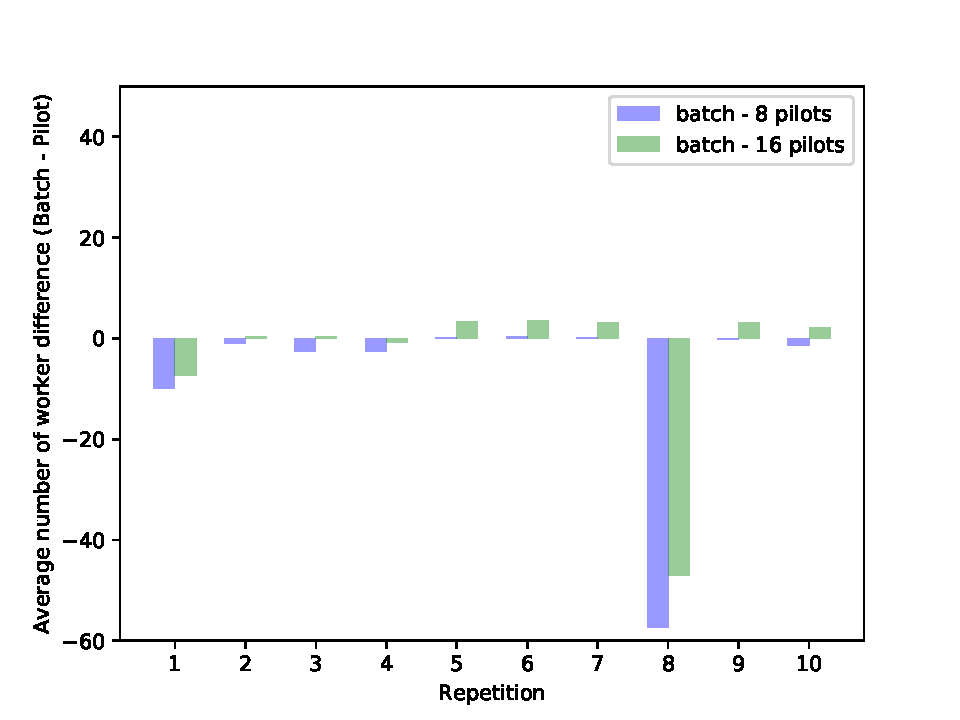
\includegraphics[width=\textwidth]{figures/spa/nworkers_4_beluga}
		\caption[]%
		{{\small Configuration 4}}
		\label{fig:spa:nwbeluga4}
	    \end{subfigure}
	    \caption{\small  The difference in average workers on B\'eluga
	    between batch and pilots for all configurations and repetitions.
	    Positive values mean that batch had more workers than pilots, that
	    is, pilots did not improve queuing times.}
	    \label{fig:spa:nworkersbeluga}
	\end{figure*}
	\begin{figure*}
	    \centering
	    \begin{subfigure}[b]{0.475\textwidth}
		\centering
		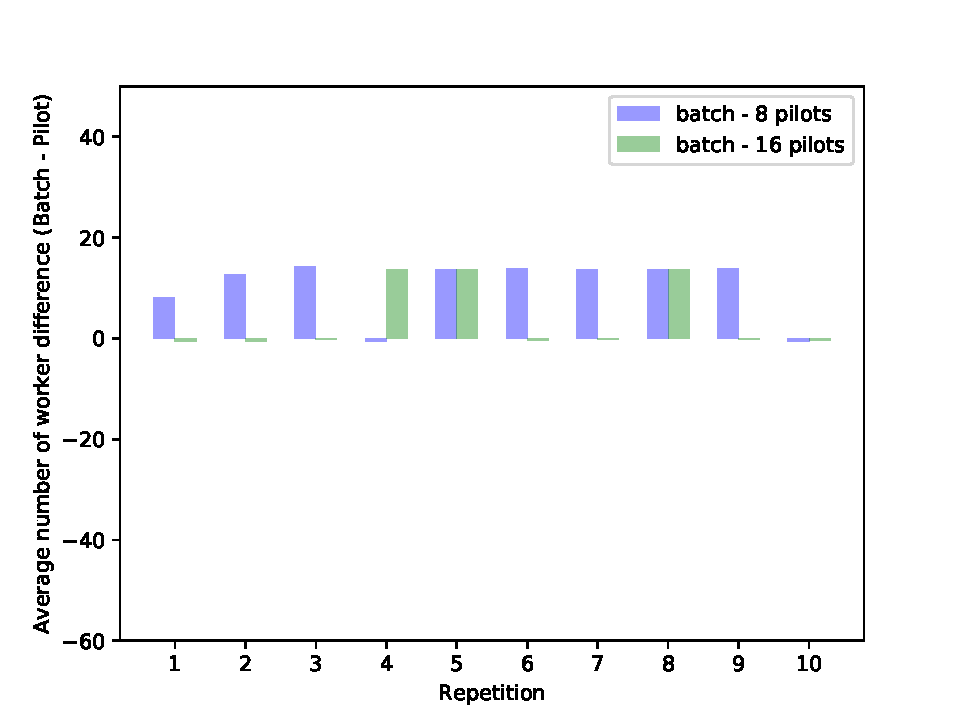
\includegraphics[width=\textwidth]{figures/spa/nworkers_1_cedar}
		\caption[]%
		{{\small Configuration 1}}
		\label{fig:spa:nwcedar1}
	    \end{subfigure}
	    \hfill
	    \begin{subfigure}[b]{0.475\textwidth}
		\centering
		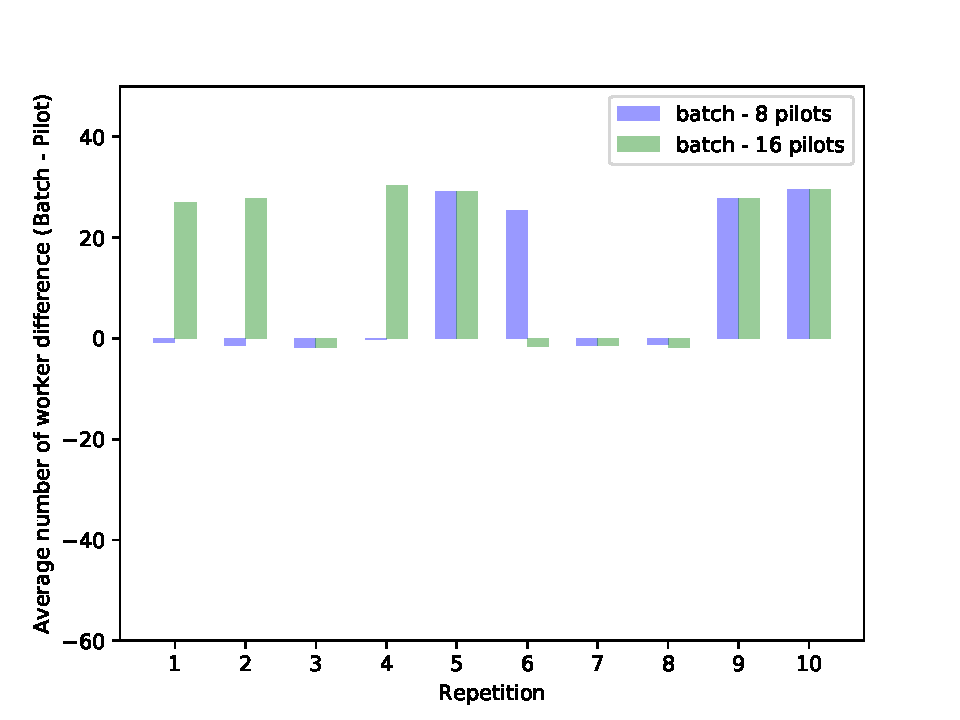
\includegraphics[width=\textwidth]{figures/spa/nworkers_2_cedar}
		\caption[]%
		{{\small Configuration 2}}
		\label{fig:spa:nwcedar2}
	    \end{subfigure}
	    \vskip\baselineskip
	    \begin{subfigure}[b]{0.475\textwidth}
		\centering
		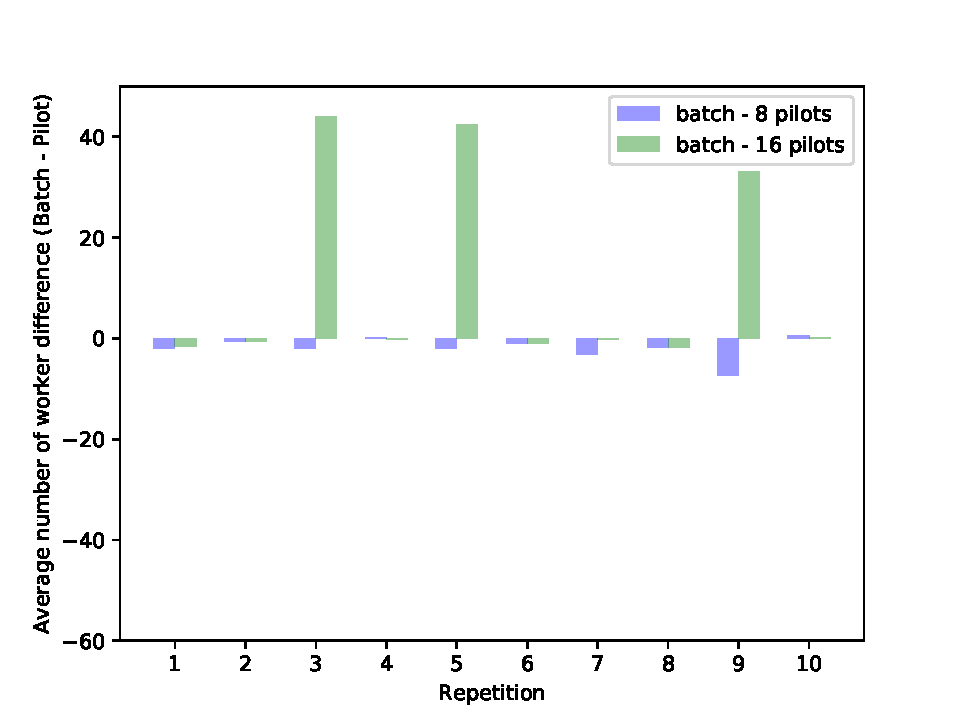
\includegraphics[width=\textwidth]{figures/spa/nworkers_3_cedar}
		\caption[]%
		{{\small Configuration 3}}
		\label{fig:spa:nwcedar3}
	    \end{subfigure}
	    \quad
	    \begin{subfigure}[b]{0.475\textwidth}
		\centering
		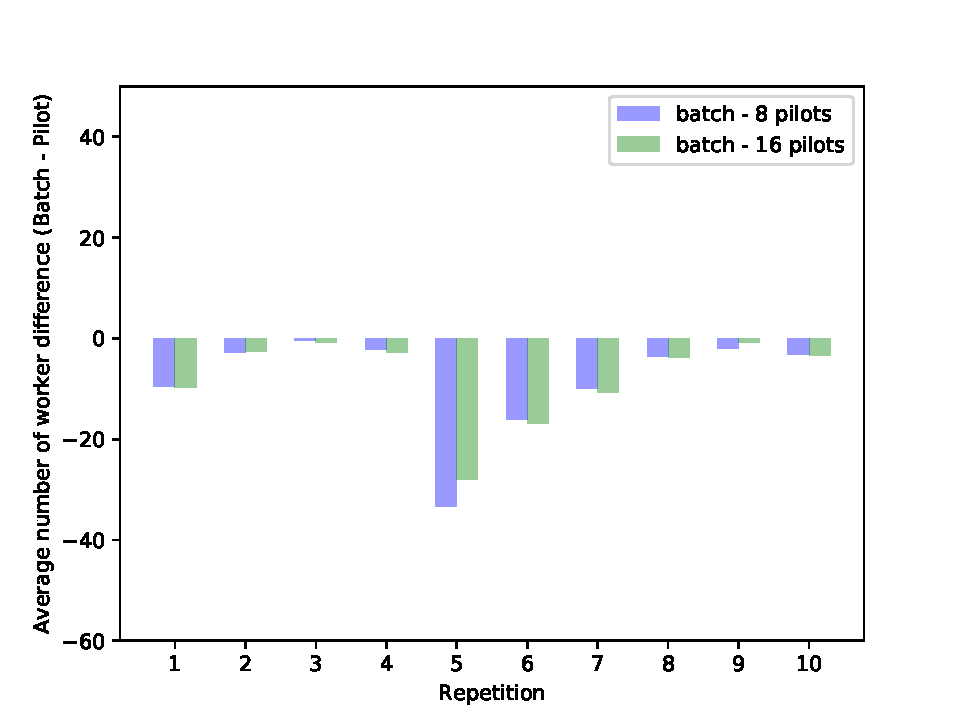
\includegraphics[width=\textwidth]{figures/spa/nworkers_4_cedar}
		\caption[]%
		{{\small Configuration 4}}
		\label{fig:spa:nwcedar4}
	    \end{subfigure}
	    \caption{\small The difference in average workers on Cedar between
	    batch and pilots for all configurations and repetitions. Positive
	    values mean that batch had more workers than pilots, that is, pilots
	    did not improve queuing times.}
	    \label{fig:spa:nworkerscedar}
	\end{figure*}
    
    \begin{table}                                                                    
	\centering                                                                       
	\begin{tabular}{c|c|c|c|c}                                                             
	    {} & \multicolumn{2}{c}{B\'eluga} & \multicolumn{2}{c}{Cedar}\\
	\rowcolor{headcolor}                                                             
	Configuration & 8 pilots & 16 pilots & 8 pilots & 16 pilots\\
	
	\hline                                                                           
	1 & 0.949 & 0.932 & 0.724 & 0.874\\
	
	2 & 0.988 & 0.916 & 0.836 & 0.826\\
	
	3 & 1.458 & 1.369 & 0.941 & 0.964\\
	4 & 0.970 & 0.891 & 1.049 & 1.068\\
	\end{tabular}                                                                    
	\setlength{\belowcaptionskip}{-10pt}                                             
	\caption{Average speedup of pilots for each configuration}                                                    
	\label{table:spa:speedup}                                                            
    \end{table} 
    
    
    
	\begin{figure*}
	    \centering
	    \begin{subfigure}[b]{0.475\textwidth}
		\centering
		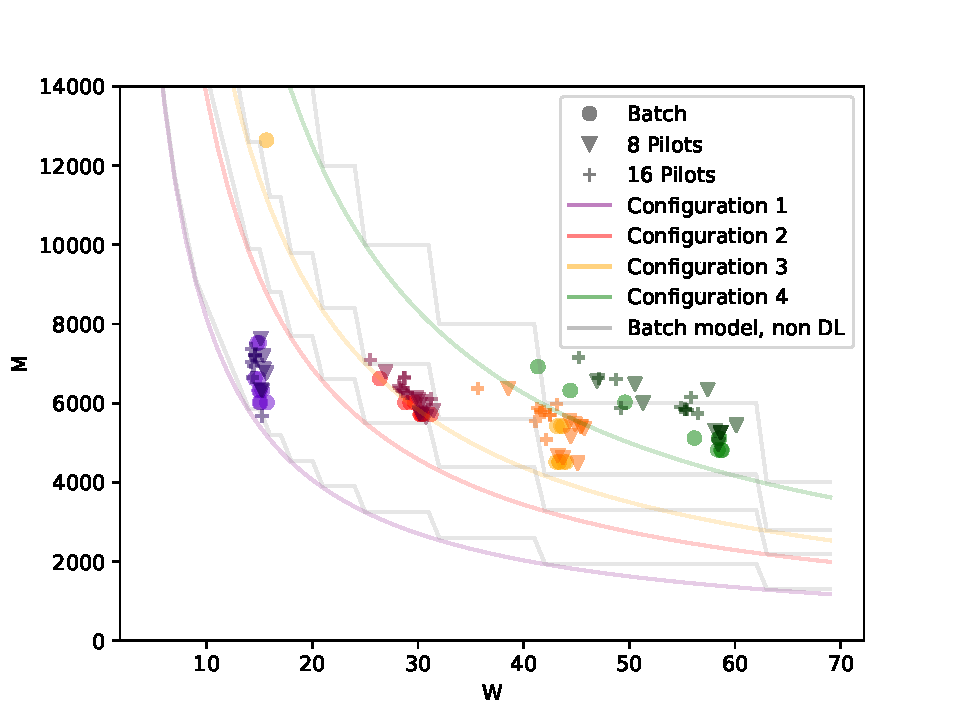
\includegraphics[width=\textwidth]{figures/spa/mw_beluga}
		\caption[]%
		{{\small Beluga}}
		\label{fig:spa:mwbeluga}
	    \end{subfigure}
	    \hfill
	    \begin{subfigure}[b]{0.475\textwidth}
		\centering
		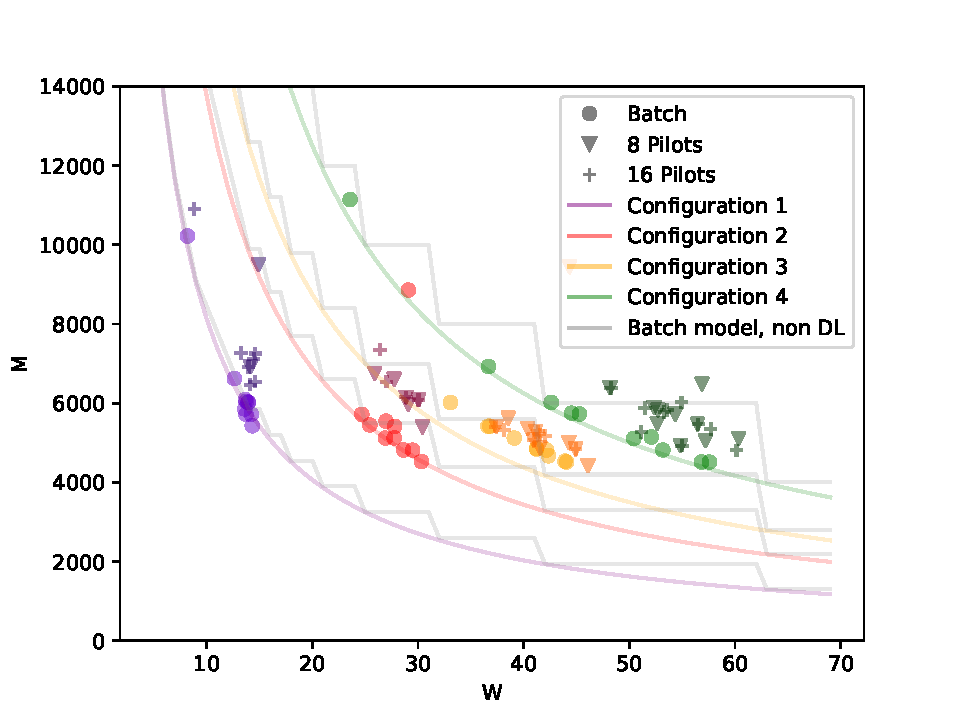
\includegraphics[width=\textwidth]{figures/spa/mw_cedar}
		\caption[]%
		{{\small Cedar}}
		\label{fig:spa:mwcedar}
	    \end{subfigure}
	    \caption{\small The relation between makespan and average number of
	    workers as calculated using Equation~\ref{eq:spa:avgw}. Trendline
	    denotes the expected makespan given the average number of workers
	    given a certain configuration}
	    \label{fig:spa:mwall}
	\end{figure*}
    
    \section{Discussion}\label{spa:sec:discussion}
    
    %SPA vs other frameworks.
    
    %Technical overhead of using pilots + an overlay cluster over a cluster.
    Pilots do not appear to provide any performance advantage over batch
    scheduling when deploying Apache Spark overlay clusters on HPC. This can be
    due to a few reasons. The queuing time for batch and pilots were similar,
    which can be an indication that we were just lacking the right level of
    priority to have been scheduled immediately. In the instances where batch
    was found to be significantly slower, it might have been case that we had
    obtained the necessary priority level but there were not enough resources
    available to be scheduled.
    
    It was also found that having 16 pilots was generally slower than 8 for the
    same configuration. This was particularly the case on B\'eluga. We suspect
    this might be related to the number of Slurm jobs permitted for a user on
    the backfill queue. For all configurations, we ran batch, 8 pilots and 16
    pilots concurrently. This would have resulted in 25 Slurm jobs trying the
    access the queue concurrently. On B\'eluga, the max number of jobs in the
    backfill queue is configured to a total of 10 jobs. For 16 nodes, this would
    at best be only 62.5\% of the pilots being scheduled at a given time if all
    resources are available. The next 6 jobs would then have to wait 3 minutes
    before having an opportunity to enter the backfill. Cedar, on the other
    hand, permits 40 user jobs to be backfilled at a given time. Therefore, on
    Cedar, all concurrent Slurm jobs had an opportunity to be backfilled at the
    same time, which may explain why this behaviour is more apparent on
    B\'eluga. Furthermore, while both pilot configurations could be placed in
    B\'eluga's low memory nodes, batch requests had to be placed on B\'eluga's
    medium memory nodes. B\'eluga has 172 low memory nodes and 516 mid memory
    nodes. As pilots would get priority for the low memory nodes first and low
    memory nodes are less frequent than medium memory nodes, it is possible that
    this may have increased the overall queuing times of the pilots. However,
    Cedar's basic node has enough memory to for all batch and pilot
    configuration, therefore, this could not have affected queuing times in
    Cedar.
    
    Although queuing time is largely responsible for makespan variations, it is
    not always entirely responsible for the differences. Sometimes there are
    errors related to executors not properly starting. These occurrences lead to
    the application being processed entirely with a smaller number of available
    executors. As the task delay added assumes the maximum number of parallel
    workers, functioning with less total workers will significantly affect
    makespan. However, as seen in Figure~\ref{fig:spa:mwall}, pilots are slower
    even with the same amount of average workers. A potential reasoning for this
    may be the worker registration delay and the time required to transfer data
    over after the application has already started. In batch scheduling, all
    workers are started in parallel and the data is transferred automatically at
    the beginning of the pipeline, as the maximum amount of parallelism is
    available at driver start time. Pilots, on the other hand, may start workers
    in parallel, but not necessarily all will be started at the same time (i.e.
    delays in starting the workers once resources have been allocated). This
    means that the entire workflow may suffer the impacts of starting workers in
    sequence rather than in parallel. Moreover, there would also be a delay with
    respect to transferring data from workers to newly added workers. Therefore,
    it is only natural that pilots would have a bit more overhead than batch
    given the same queuing time should pilots not all commence at once, despite
    transferring the same amount of data. Furthermore, the pilot scripts also
    have some startup overhead as all pilots start a master, a worker
    (registered to the main master) and attempt to start a driver. Batch needs
    only start a single master and attempts to start a driver only once.
    
    The motivation to use pilots, however, is dynamic scheduling on HPC
    clusters. While we investigated the queuing time differences with respect to
    differences in available resources, the wall-times were kept static. Had
    wall-times been underestimated to the point where the Slurm jobs would
    terminate prior to application completion, pilots might have been preferable
    to batch as batch scheduling has no mechanism to restart. Even if such a
    mechanism was in place, the entire cluster would be shutdown and need to
    restart, which has additional overheads. With pilots, as long as there is at
    least one pilot alive, it would be possible to maintain the cluster and add
    additional pilots. Spark provides built-in fault-tolerance for not only the
    workers, but the master and driver as well. However, it is also likely that
    with faster queuing times, all resources would be allocated at the same
    time. If wall-times were to be underestimated, in this case, checkpointing
    and restarting the entire application from the last checkpoint would be the
    only option. This too has limitations as the last checkpoint may not be
    recent, necessitating significant amounts of recomputation. It might even be
    desirable to have many small resource requests in such a scenario, as it
    becomes less likely for all pilots to start at once as they become more
    numerous, as can be seen with 16 pilots when compared to 8. This would allow
    for more chances for the application to reach completion without failing
    entirely.
    
    Many failures can be found, particularly in regard to the pilots. Most of
    these have been a result of Spark failing to start properly. The driver
    either would not return a submission ID after being started, or would remain
    in \texttt{SUBMITTED} status until the wall-time expiration, having not
    processed any data. As these errors become fewer with increased resources,
    it is possible they are entirely related to lack of resources. Furthermore,
    it may also explain why batch submission is more frequently successful. Not
    only are all the workers that were requested available when the pilot begins
    running, but batch also has one extra executor available thanks to the
    driver process running directly on the process which had created it, rather
    than on a worker process. Conversely, it is not only the pilot applications
    that fail; batch applications do experience some failures as well. It can be
    seen in Figure~\ref{fig:spa:makespansbeluga} that the batch application
    failed twice: once in Configuration~2 and the other in Configuration~4. In
    both cases, the reason for failure was the same: lack of available resources
    despite all executors having been assigned. These failures might be due to
    running on a shared HPC cluster. Either the resources were down, or other
    users might have been using them, resulting in the resources being
    unavailable to our application.
    
    Running a Spark cluster atop of a Slurm allocation complicates debugging,
    particularly if the application runs in cluster mode. Spark worker logs,
    unless saved to network storage, become unavailable after program execution.
    Although the worker UI is available during program execution, a user must
    manually create an SSH tunnel to each worker node to gain access to them. An
    option is to save the logs to a shared network storage for future access.
    This effectively slows down the application as the network file system is
    typically a slower storage than local storage.
    
    When running in client mode, the driver output ends up in standard
    output/error. However, in cluster mode, the driver output is found stored
    within the worker logs, which means the driver logs are also inaccessible
    without worker logs being written to network storage. Some HPC clusters may
    have a file limit for users, meaning that the user must be sure that these
    logs coupled without other stored data does not exceed the file limit.  
    
    \section{Conclusion}\label{spa:sec:conclusion} Pilots do not provide
    significant advantage over batch systems to run Apache Spark applications on
    HPC clusters. This is affected by the overhead of dynamically adjusting the
    cluster size and the fact that queuing time of the batch applications took
    as long as the pilots. These results, however, are to an extent
    cluster-dependent. It is expected that as the number of resources requested
    increases, the speedup provided by pilots will increase. Furthermore, users
    executing on a smaller cluster may experience greater speedups using the
    same resource configuration. Our resource requirements and cluster size,
    however, match typical configurations currently available to scientific
    communities.
    
    Although obtained with Apache Spark, this result is likely to generalize to
    other implementations of overlay clusters. Conversely, our experiments do
    \emph{not} imply that pilot jobs are not useful on HPC clusters in the
    absence of overlay clusters. Most pilot job implementations in fact include
    an overlay scheduler, which allows for various types of optimization
    including dealing with fine task granularity or enforcing data locality.
    Pilot jobs naturally remain useful in that respect.
    
    Pilots are meant to allow for underestimation of resources, particularly
    wall-time, which would not be known to the user prior to execution. In its
    current state, \texttt{SPA} is not able to evaluate that functionality.
    Further experiments on master fault-tolerance, driver recovery, and
    checkpointing will need to be conducted to determine if pilot jobs are even
    a viable solution for Spark applications running on HPC.
    
    Currently, as client mode is not available in Spark Standalone clusters for
    PySpark applications, using pilots on HPC would be limited to non-Python
    applications until there is a solution for Standalone mode.